% main.tex
\documentclass[12pt]{article}



% Import formatting & packages
% preamble.tex
\usepackage[a4paper, margin=2.5cm]{geometry}  % Page size & margins
\usepackage{graphicx}   % Figures
\usepackage{subcaption} % Defines the subfigure environment
\usepackage{booktabs}   % Professional tables
\usepackage{amsmath}    % Math symbols & equations
\usepackage{amssymb}    % More math symbols
\usepackage{hyperref}   % Hyperlinks
\usepackage{cleveref}   % Smart references
\usepackage{enumitem}   % Customizable lists
\usepackage{float}      % Better table/figure placement
\usepackage[utf8]{inputenc}  % Ensure Overleaf uses UTF-8 encoding
\usepackage{csquotes}   % Improved quotation formatting
\usepackage{tabularx}
\usepackage{tabularray}
\usepackage{tikz}
\usetikzlibrary{shapes.geometric, arrows}
\usepackage{pgfplotstable,siunitx,xfp}
\pgfplotsset{compat=1.18}
\usepackage{siunitx}   % \num, rounding/formatting
\usepackage{xfp}       % or expl3; xfp gives \fpeval
\usepackage{titling} 
\usepackage{verbatim} % for \verbatiminput
\usepackage{catchfile}
\usepackage{multirow}
\usepackage{booktabs}
\usepackage{array}
\usepackage{setspace}


% Bibliography
\usepackage[backend=biber, style=authoryear, sorting=nyt]{biblatex}  
\addbibresource{references.bib}  % Link to your Zotero export

% Section number depth
\setcounter{secnumdepth}{3}

% Table & figure captions
\usepackage[labelfont=bf]{caption}  

 % Word count command
\newcommand{\wordcount}{%
  % Run texcount on the main document (jobname.tex)
  %  - stdout -> \jobname.wc
  %  - stderr (warnings) -> nul (ignored)
  \immediate\write18{texcount -inc -sum -0 -template={SUM} \jobname.tex > \jobname.wc 2> nul}%
  % Read the result from the temporary file:
  \CatchFileDef{\wcresult}{\jobname.wc}{}%
  \mbox{\wcresult\unskip}%
}









% Auto-generated values from R
\input{values}


\begin{document}

%TC:ignore
\begin{titlepage}
  \begin{center}
    \vspace*{1cm}

    % University + document type
    {\Large UNIVERSITEIT UTRECHT\par}
    \vspace{0.5cm}
    {\large MASTER THESIS\par}

    \vspace{2cm}

    % Title
    {\Huge \textbf{Addressing the Cold Start Problem in AI-Assisted Systematic Reviews}\par}
    \vspace{0.5cm}
    {\LARGE
      Getting started when evidence is scarce \par
    }

    \vspace{2.5cm}

    % Author(s)
    {\large \textbf{Author:}\par}
    \vspace{0.2cm}
    {\large Timo van Ommeren\par}

    \vspace{1cm}

    % Supervisor(s)
    {\large \textbf{Supervisors:}\par}
    \vspace{0.2cm}
    {\large Prof. dr. A.G.J. (Rens) van de Schoot, Lauke Stoel\par}

    \vspace{1.5cm}

    % Programme / degree line (adapt as you like)
    {\large
      MSc Methodology and Statistics for the Behavioural,\\
      Biomedical and Social Sciences\par}

    \vspace{0.5cm}

    % Host department / organisation (mirroring "Ministry of Health..." line)
    {\large Methodology Department, Utrecht University\par}

    \vfill

    % Logo
    
\includegraphics[width=0.2\textwidth]{images/Utrecht_University.png}

    \vspace{0.8cm}

    % Date and word count
    {\large \today\par} {\large Word count: \wordcount}

  \end{center}
\end{titlepage}
%TC:endignore


\section{Introduction}

\subsection{The framework: AI-assisted systematic reviews}

Researchers and practitioners are continually challenged to base their decisions on the latest scientific evidence \parencite{sackett1996evidence, subbiah2023next, sheridan2016achievements, chalmers2002brief}. This requires critically reviewing increasingly large bodies of literature \parencite{jinha2010article, bornmann2015growth}. To that end, systematic reviews and meta-analyses were developed as rigorous methods of summarizing scientific literature \parencite{grant2009typology, brignardello2025systematic, borenstein2021introduction, kicinski2015publication}. However, systematically reviewing large bodies of literature can be time-consuming. In particular, screening titles and abstracts to identify relevant papers is often a major bottleneck limiting the practical applicability of systematic reviews \parencite{nussbaumer2021resource, bastian2010seventy, borah2017analysis}.

Fortunately, recent advances in machine learning have produced tools that assist researchers in screening papers by prioritizing the most relevant papers for screening first \parencite{van2021open, ouzzani2016rayyan, ge2024leveraging, dos2023usefulness}. One such tool is \textit{ASReview}, an open-source software package for artificial intelligence (AI)-assisted systematic reviews \parencite{van2021open, asreviewvs2jonathan}. ASReview uses active learning models to iteratively learn from the user's screening decisions and adaptively prioritize the most relevant papers for screening (see \autoref{figure_1}). AI-assisted screening can significantly reduce the time and effort needed to conduct systematic reviews and may even help identify more relevant papers compared to screening without the help of AI \parencite{teijema2025large, byrne2024impact, ferdinands2023performance, van2025hunt}. 

\begin{figure} [b!]
  \centering
  \includegraphics[width=0.9\textwidth]{results/figure_1_Brouwer\_2019.png}
  \caption{A recall plot of a random run of AI-assisted simulated screening of the systematic review by \textit{Brouwer\_2019}, compared to manual screening. One example of a relevant abstract was provided before simulating screening.}
  \label{figure_1}
\end{figure}

\subsection{The cold start problem}

%what is the cold start in AI-assisted systematic reviews 
AI-assisted screening tools such as ASReview require an example of a relevant paper before the start of screening to be able to assist in screening from the very start \parencite{van2021open,teijema2025large}. More specifically, ASReview classifies papers as relevant (1) or irrelevant (0). The AI-model thus requires at least one paper in each class to predict the probability of relevance for unscreened papers and order them accordingly. If no examples of papers have been provided before the start of screening, ASReview will present papers at random until at least one relevant and one irrelevant paper have been found (see \autoref{figure_1}). This known as the cold start problem \parencite{panda2022approaches}. 

In practice, irrelevant papers are abundant and so will be found instantantly. In contrast, finding a relevant paper through random search may take a long time, especially when the percentage of relevant papers returned by a systematic search is low (see \autoref{tab:SYNERGY} for these percentages for 23 published systematic reviews, and see \cite{nussbaumer2021resource, borah2017analysis} for screening time estimations). Thus, in practice only a relevant paper is necessary before the start of screening (though also providing an irrelevant paper does help to narrow the search space).

Interestingly, screening papers at random until a relevant record is found does not result in more papers needing to be screened to find \textit{all} relevant papers \parencite{oude2023can}. Therefore, the cold start problem in AI-assisted screening tools only applies if AI-assisted screening is needed from the very start of screening. 

\bigskip

We may thus define the scope of the problem more precisely:

\begin{mdframed}[linewidth=3pt, linecolor=black, 
                 topline=false, bottomline=false, rightline=false,
                 innerleftmargin=10pt]
\textbf{Problem statement:} The cold start problem poses a practical barrier to AI-assisted screening when (1) no relevant papers are available before the start of screening, and (2) AI-assisted screening is needed from the very start of screening.
\end{mdframed}

% \begin{tcolorbox}[colback=gray!10, colframe=gray!50]
% \textbf{Problem statement:} The cold start problem poses a practical barrier to AI-assisted screening when (1) no relevant papers are available before starting screening, and (2) adequate starting performance is crucial.
% \end{tcolorbox}


\subsection{The niche: rapid reviews in times of crisis}

One setting in which AI-assisted screening may be necessary from the very start of screening, and no relevant records are available, is when conducting rapid reviews in times of crisis (for an introduction to rapid reviews, see \cite{garritty2025rapid, haby2024best, smela2023rapid}). For example, during the COVID-19 pandemic some rapid reviews were reportedly conducted within 10 days and some even within a few hours \parencite{tricco2020rapid}. This means that during a crisis situations it may not be possible to continue screening until all relevant records have been found (deciding when to stop screening when using AI is a non-trivial problem in and of itself, see \cite{boetje2024safe, bron2025using}). Evidently, in this case it is desirable to have AI-assisted screening from the very start. 

Yet during a crisis situation no examples of relevant records may be available before the start of screening. At the beginning of the pandemic, for example, experts had to rely on indirect evidence from other pandemics and respiratory diseases \parencite{kurzer2023follow, brooks2020psychological}. In this case, indirect evidence may be used to initialize the AI-model to have AI-assisted screening from the very start. However, this may cause the screener to become stuck on an unrepresentative subset of the relevant papers (a similar phenomenon has been noted in computational psychiatry, \cite{rosbach2026stuck}). That is, literature directly applicable to the problem at hand may be available, but, becuase the screener is unaware of this fact they may end up in what we may call an \textbf{epistemic ecochamber}. 

Therefore, the quality of rapid reviews in times of crisis could be improved by developing an approach which initializes AI-assisted screening tools without the use of any existing literature. 

% A rapid review is a quicker alternative to a systematic review, but is less rigorous and complete \parencite{haby2024best, smela2023rapid, tricco2015scoping}. For example, a rapid review may search fewer databases, restrict searches to particular languages and dates, and employ single-reviewer screening. These adjustments increase the speed of a review, but also the risk of bias \parencite{tricco2017rapid, kelly2016quality, marshall2019rapid}. 

% The risk of bias is particularly present if there is time pressure from stake-holders. During the COVID-19 pandemic, for example, some rapid reviews were reportedly conducted within 10 days and some even within a few hours (\cite{tricco2020rapid}, compared to the usual 1-6 months advised by \cite{garritty2025rapid} and average 3.2 months found by \cite{abou2016methods}). The increased time pressure was partially adressed by the use of AI-assisted screening tools \parencite{fdAIprogrammaUtrecht}. However, whether this biased the conclusions of the resulting reviews is unclear \parencite{haby2024best, tricco2020rapid}.

% One source of bias may have been the examples (or lack thereof) used to train the AI-model before the start of screening. In emerging health crises such as the COVID-19 pandemic it may not be clear what constitutes as relevant evidence. For instance, at the beginning of the pandemic, experts had to rely on indirect evidence from other pandemics and respiratory diseases \parencite{kurzer2023follow, brooks2020psychological}. This may have resulted in one of two scenarios: either no examples were used to train the AI model before screening, which limited the total number of relevant papers found and potentially biased the results, or unrepresentative previous research was used to train the AI model before screening, leading to an unrepresentative subset of relevant papers being found and thereby biasing the results \parencite{rosbach2026stuck}.




\subsection{The proposed solution: eligibility criteria and LLMs}

A possible solution to the cold start problem is to use a systematic review's eligibility criteria to initialize the AI model. When conducting a systematic review, eligibility criteria are defined before screening to provide the screeners with the criteria for including or excluding papers in the review (\cite{cochraneChapterDefining}, for an example see \autoref{sec: LLM generated abstracts}). Therefore, a cold start may be avoided by providing the eligibility criteria as an example of an abstract of a relevant paper to the AI model before the start of screening. 

Starting performance may be further increased by using large language models (LLMs). Specifically, based on the eligibility criteria of a systematic review, an LLM can be instructed to generate an (hallucinated) example of the title and abstract as of a relevant paper. Providing this generated title-abstract pair at the start of screening may prove to increase starting performance further than using the eligibility criteria directly. The LLM may add information over and above the eligibility criteria by leveraging its training data \parencite{zhang2025cold, bachmann2025adaptive}. However, the use LLMs may also add unncessary steps or even negatively impact starting performance by adding noise \parencite{gartlehner2025responsible, sollini2025human}.

\subsection{Objectives}

Given the problem and proposed solution above, the main goals of the present study are to investigate whether:

\begin{enumerate}
  \item The number of relevant papers found at the start of AI-assisted screening can be increased by providing a systematic review’s eligibility criteria as an example of a relevant abstract compared to providing no examples at all (i.e. a cold start). 
  \item The number of relevant papers found at the start of AI-assisted screening can be increased further providing an (hallucinated) title-abstract pair generated by an LLM based on a systematic review’s eligibility criteria.
\end{enumerate}

\newpage

\section{Methodology}

To address the research questions above, we will simulate the screening of papers by relevance of published systematic reviews using ASReview.  

\subsection{Simulation design}

To simulate the AI-assisted screening of papers, we will use 21 datasets; each containing the title and  abstract, and relevance label (0 or 1) of all the papers screened for published systematic reviews (from the SYNERGY collection \cite{de2023synergy}. See \autoref{tab:SYNERGY} for the metadata of each systematic review, e.g., number of records screened and percentage of relevant papers.). Since these systematic reviews were conducted without the help of AI-assisted screening, each paper obtained from their systematic searches has been screened and labelled. This allows us to simulate the same screening decisions but with the help of ASReview and estimate the time and effort saved compared to manual screening (for related simulation studies see \cite{teijema2025large, byrne2024impact, ferdinands2023performance}). 

Since the cold start problem effects starting performance only, the current study will simulate the screening of the first 100 papers of each dataset only. Starting performance will be measured by counting the number of relevant papers retrieved in the first 100 papers screened (i.e., $x = \frac{count \space relevant}{total \space screened}$). Two sequential configurations of ASRview are used: the first queries papers at random until at least one relevant and one irrelevant paper have been found and ASReview's classifier can be trained. Next the U4 configuration is used for the remainder of the screening process. Notably, however, in all conditions except for the cold-start condition, the first configuration is effectively skipped since at least one relevant paper is provided before screening begins and irrelevant papers are plentiful in all systematic reviews. See \parencite{asreviewvs2jonathan} for a detailed description of the U4 configuration.

To address the research questions above, four different ways of initialization the AI-model before the start of screening will be compared: 

\medskip

\noindent Four starting conditions are compared:
\begin{enumerate}[label=\textbf{\Alph*.}]
    \item \textit{Eligibility criteria} — the eligibility criteria of the systematic review are provided directly to ASReview as an example of a relevant paper.
    \item \textit{LLM-generated} — the eligibility criteria are first passed to GPT-4o-mini\footnote{OpenAI's gpt-4o-mini model is instructed via a DSPY module for dynamic prompt generation in each run \parencite{khattab2023dspy}}, which is prompted to generate an (hallucinated) title and abstract of a plausibly relevant paper. These are then provided to ASReview. This is repeated every run.
    \item \textit{Cold start} — no example is provided before screening; ASReview begins screening without initialisation.
    \item \textit{Actual paper} — one paper from the set of relevant papers is sampled (with replacement across runs) and provided to ASReview as an example.
\end{enumerate}

% Conditions A and B constitute the experimental manipulations of interest, while C serves as the primary contrast and D as an upper-bound reference.

% As described above, the first type of starting condition uses the (A) \textit{eligibility-criteria} of the systematic review directly as an example of an abstract of a relevant paper with which to initialise ASReview. In the second starting condition the eligibility criteria are provided to (B) an \textit{LLM} first. To be precise, OpenAI's GPT-4o-mini model is prompted to generate an (hallicunated) title and abstract pair of a relevant paper based on the eligibility criteria\footnote{OpenAI's gpt-4o-mini model is instructed via a DSPY module for dynamic prompt generation in each run \parencite{khattab2023dspy}}. This title and abstract are then provided to ASReview as an example of a relevant paper.

% The two types of starting conditions described above are compared to two other starting conditions. The first is the contrast of interest: a (C) \textit{cold-start}, in which case no papers are provided to ASReview before to the start of screening. The last type of starting condition uses an \textit{actual paper} as an example. Specifically, one relevant paper is sampled from the set of papers labeled as relevant to the systematic review at hand (with replacement between runs) and provided to ASReview before screening.

% Finally, the eligibility criteria of the systematic reviews are manually manipulated in several ways to investigate whether this affects starting performance. Specifically, the alterations made are: the presence of exclusion criteria, expansion of abbreviations, and expansion of generic terms using MeSH\footnote{For example, "rodents" may be expanded to include hyponyms such as "mice" and "rats", and "Wilson's disease" to include synonyms such as "Progressive Lenticular Degeneration"}. 

The total number of simulation runs is 4 (conditions) x 21 (systematic reviews) x 2 (manipulated vs. unmanipulated eligibility criteria) = 184 runs. FIX!!!

Before conducting a full simulation study, some exploratory simulations will be conducted which screen \textit{all} the papers from the Appenzeller-Herzog\_2019 and Brouwer\_2019 datasets only. 


\subsection{Analysis plan}

Starting performance will be compared between the four conditions visually using a boxplot and statistically using a linear model with bootstrapped SEs. Starting performance is defined as the number of relevant papers successfully retrieved from among the first 100 papers screened. However, in some simulation runs all relevant papers may be retrieved before a 100 papers is screened. In this case screening would stop prematurely. 

To account for the fact in some runs less than a 100 papers may be, the total number of papers screened will be included in the model. Furthermore, it is expected that most of the variance in starting performance will be explained by differences in performance of ASReview between systematic reviews \parencite{teijema2025large}. Therefore, a dummy variable controlling differences between the simulated systematic reviews will also be included in the model. Finally, an additional analysis will be conducted to explore the impact of manually manipulating the eligibility criteria. Some initial simulations comparing overall performance were also conducted.  

%\clearpage




\section{Results}



% Runs showed a clear difference in the number of relevant papers found within the first 100 papers screened between when no examples of relevant papers were provided before the start of screening (i.e., a cold start) and the other three starting conditions (see \autoref{figure_2}). However, no clear differences between the other three conditions were apparent. There also appeared to be large differences in the number of relevant papers found between runs, in particular when no examples of relevant papers were provided before the start of screening. 

% Finally, screening was simulated 27 times for each of the 4 starting conditions for all the 21 systematic reviews in the SYNERGY dataset. For 6 of these systematic reviews, the resulting recall plots are shown in \autoref{fig:aggregate-recall-plots}. The plots demonstrate the heterogeneity in both the average and variance of screening performance across the systematic reviews. Some plots, such as Leenaars\_2020, show little average difference between the four conditions, while others, such as Radjenovic\_2013, show a clear difference. Similarly, some plots, such as Nelson\_2002, show little variance, while others, such as Muthu\_2021, show considerable variance. Finally, some plots, such as Brouwer\_2019, show that beginning with an actual paper before screening can result in outliers, with significantly fewer relevant papers being identified than when usually starting with an actual paper when screening for that systematic review. 

% The MODEL RESULTS OF THE SPECIFIC COMPARISONS


% \begin{figure}
%   \centering
%   \begin{subfigure}[t]{0.48\textwidth}
%       \centering
%       \includegraphics[width=1\linewidth]{results/figure_2_Appenzeller-Herzog\_2019.png}
%       \caption{Appenzeller-Herzog\_2019}
%       \label{fig:full-recall-plot-appelneller-herzog}
% %\clearpage
%   \end{subfigure}
%   \hfill
%   \begin{subfigure}[t]{0.48\textwidth}
%       \centering
%       \includegraphics[width=1\linewidth]{results/figure_2_Brouwer\_2019.png}
%       \caption{Brouwer\_2019}
%       \label{fig:full-recall-plot-brouwer}
%   \end{subfigure}
%   \caption{Randomly chosen runs of AI-assisted simulated screening of Appenzeller-Herzog\_2019 (left) and Brouwer\_2019 (right).}
%   \label{figure_2}
% \end{figure}







\begin{figure}[htbp]
  \centering
  \captionsetup[subfigure]{skip=2pt, font=footnotesize}
  \begin{subfigure}[t]{0.48\textwidth}
    \includegraphics[width=\linewidth]{results/individual_runs/individual_runs/Appenzeller-Herzog_2019/figure_3_run_1_IVs_1_100_0.0.pdf}
    \caption{Appenzeller-Herzog (2019)}
    \label{fig:recall-plot-appenzeller-herzog}
  \end{subfigure}\hfill
  \begin{subfigure}[t]{0.48\textwidth}
    \includegraphics[width=\linewidth]{results/individual_runs/individual_runs/Brouwer_2019/figure_3_run_1_IVs_1_100_0.0.pdf}
    \caption{Brouwer (2019)}
    \label{fig:recall-plot-brouwer}
  \end{subfigure}

  \caption{Single simulation runs of the Appenzeller-Herzog\_2019 (left) and Brouwer\_2019 (right) datasets, illustrating the effect of
    initialisation condition on early screening performance. Colours indicate initialisation
    condition:
    \textcolor[rgb]{0.902,0.624,0.000}{cold start},
    \textcolor[rgb]{0.835,0.369,0.000}{eligibility criteria},
    \textcolor[rgb]{0.000,0.447,0.698}{LLM}, and
    \textcolor[rgb]{0.000,0.620,0.451}{actual paper}.}
  \label{fig:individual-runs}
\end{figure}



\begin{figure}[p]
  \centering
  \captionsetup[subfigure]{skip=2pt, font=footnotesize}

  % Row 1
  \begin{subfigure}[t]{0.48\textwidth}
    \includegraphics[width=\linewidth]{results/aggregate_recall_plots/figure_4_Appenzeller-Herzog_2019.pdf}
    \caption{Appenzeller-Herzog (2019)}
  \end{subfigure}\hfill
  \begin{subfigure}[t]{0.48\textwidth}
    \includegraphics[width=\linewidth]{results/aggregate_recall_plots/figure_4_Brouwer_2019.pdf}
    \caption{Brouwer (2019)}
  \end{subfigure}

  \par\vspace{4pt}

  % Row 2
  \begin{subfigure}[t]{0.48\textwidth}
    \includegraphics[width=\linewidth]{results/aggregate_recall_plots/figure_4_Leenaars_2019.pdf}
    \caption{Leenaars (2019)}
  \end{subfigure}\hfill
  \begin{subfigure}[t]{0.48\textwidth}
    \includegraphics[width=\linewidth]{results/aggregate_recall_plots/figure_4_Menon_2022.pdf}
    \caption{Menon (2022)}
  \end{subfigure}

  \par\vspace{4pt}

  % Row 3
  \begin{subfigure}[t]{0.48\textwidth}
    \includegraphics[width=\linewidth]{results/aggregate_recall_plots/figure_4_Muthu_2021.pdf}
    \caption{Muthu (2021)}
  \end{subfigure}\hfill
  \begin{subfigure}[t]{0.48\textwidth}
    \includegraphics[width=\linewidth]{results/aggregate_recall_plots/figure_4_Nelson_2002.pdf}
    \caption{Nelson (2002)}
  \end{subfigure}

  \par\vspace{4pt}

  % Row 4
  \begin{subfigure}[t]{0.48\textwidth}
    \includegraphics[width=\linewidth]{results/aggregate_recall_plots/figure_4_Radjenovic_2013.pdf}
    \caption{Radjenovic (2013)}
  \end{subfigure}\hfill
  \begin{subfigure}[t]{0.48\textwidth}
    \includegraphics[width=\linewidth]{results/aggregate_recall_plots/figure_4_Walker_2018.pdf}
    \caption{Walker (2018)}
  \end{subfigure}

  \caption{Aggregate recall curves for eight systematic reviews demonstrating
    substantial between-dataset variability. Thin lines show individual simulation
    runs; bold dashed lines show the condition mean. Colours indicate initialisation
    condition:
    \textcolor[rgb]{0.902,0.624,0.000}{cold start},
    \textcolor[rgb]{0.835,0.369,0.000}{eligibility criteria},
    \textcolor[rgb]{0.000,0.447,0.698}{LLM}, and
    \textcolor[rgb]{0.000,0.620,0.451}{actual paper}.}
  \label{fig:aggregate-recall-plots}
\end{figure}


\begin{figure}[htbp]
  \centering

  \begin{subfigure}{\textwidth}
    \centering
    \includegraphics[width=\textwidth]{../Report/results/spaghetti_dataset_means.pdf}
    \caption{Mean number of relevant papers found per dataset across conditions. Each line
      represents one of the 23 systematic reviews. There is substantial
      between-dataset variability ($\eta^2_p = \petadataset$).}
    \label{fig:means-per-dataset}
  \end{subfigure}

  \vspace{0.8em}

  \begin{subfigure}{\textwidth}
    \centering
    \includegraphics[width=0.72\textwidth]{../Report/results/condition_means_annotated.pdf}
    \caption{Model-estimated condition means after controlling for dataset ($\eta^2_p = \petacondition$).
      Diamonds ($\blacklozenge$) denote model-estimated means; error bars show 95\%
      bootstrapped confidence intervals. Brackets indicate the two pairwise comparisons
      of primary interest.}
    \label{fig:model-predicted-means}
  \end{subfigure}

  \caption{Number of relevant papers found across four initialisation conditions.}
  \label{fig:main-results}
\end{figure}





%This section will discuss the mean number of model predicted papers found in each condition, as well as discuss whether there are significant differences between the cold start condition and the LLM and criteria-only condition, and whether there is a significant diffeence between the LLM condition and the criteria only condition. 


% \subsection{Additional analysis on using eligibility criteria as prior}

% One alinea reporting the results of manually manipulating / enriching the elgibility criteria.

\section{Conclusion} 

The conclusion is that the cold start problem can be overcome by using the eligibility criteria of a systematic review to initialize the active learning model, and that LLM-generated examples do not improve starting performance beyond that achieved through initialisation using the systematic review's eligibility criteria criteria directly.

\begin{enumerate}
    \item The large heterogeneity between the systematic reviews screened show:
    \begin{enumerate}
        \item that the cold start problem depends on the percentage of relevant papers in the pool. For example, 21.9\% of the papers screened by Nelson\_2002 were relevant, meaning that on average a relevant paper will be identified within 5 papers screened. In contrast only 0.2\% of the papers screened by Brouwer\_2019 were relevant, meaning that an average of one relevant paper will be identified within the first 500 papers screened. Accordingly, a large difference between a cold start and the other three starting conditions is apparent for Brouwer\_2019, while for Nelson\_2002 there isn't.
        \item There are notable differences between the systematic reviews in the number of relevant papers found when using the eligibility criteria of a systematic review compared to using an actual paper. When screening the papers by Radjenovic\_2013 using the eligility criteria to initliaze the AI-model, zero relevant papers were found (25 were found on average when using an actual paper), compared to 80 relevant papers for Walker\_2018 (50 were found on average when using an average paper). 
        \item Similarly, there are a few notable differences between the systematic in the number of relevant papers found when using the eligibility criteria directly, versus generating an (hallicunated) title and abstract using an LLM first. For many systematic reviews these two starting conditions appear quite similiar. The average Appenzeller-Herzog\_2019 run when using an LLM looks like a smoothed version of when using the eligilibity criteria (with more variability too). This would fit with the conclusion that the LLM usually does not add information but simply changes the formatting. However, as mentioned above, there are a few notable differences between these conditions. For example, for Muthu\_2021 less papers were found when using an LLM. Conversly, Menon\_2022 using an LLM-generated abstract leads to more relevant papers found on average. This might be because the generic independent variable "non-acute, non-communicable, environmental exposure" is given concrete examples by the LLM such as "air pollution" (see \autoref{sec: LLM generated abstracts}) for the eligibility criteria and an example of an LLM-generated abstract).
        \item This brings us to another point. There are also differences in the variance of the number of papers found when using an actual paper between the systematic reviews. There is great variability in Walker (2018), and little variability in Leenaars\_2020. Sometimes particular papers also appear to be significantly worse at initializing the AI-model. For Brouwer\_2019 for example there appears to be one paper which leads to significantly less papers retrieved than the other papers. This paper is thus likely unrepresentative 
    \end{enumerate}
\end{enumerate}



\section{Discussion}

A factor limiting the practical application of AI-assisted systematic reviews is the `cold start' problem. More specifically, AI-assisted screening tools such as ASReview require examples of relevant literature for adequate starting performance. The practical use of AI-assisted screening tools is therefore limited in settings where (1) no examples of relevant literature are available prior to screening and (2) adequate starting performance is crucial. One example of such a setting is a crisis situation such as COVID-19, in which rapid reviews which limit rigor for speed are the standard. 

Even if one or two examples of relevant papers are  available prior to screening, using these to initialise the AI model may still lead to suboptimal starting performance. This is despite prior research showing that a single pair of relevant and irrelevant papers is sufficient for adequate starting performance \parencite{ferdinands2023performance, teijema2025large}. It may be, however, that the relevant example at hand is unrepresentative of the other paper relevant to the review. This may nudge the AI model to initially searching through mostly irrelevant papers, in what is known as an \textit{anchor effect}. ASK SIXU.

Currently, the optimal way to obtain a representative example and avoid a cold start is to ask a domain expert to provide representative examples of relevant papers. However, it may not always be feasible to contact a domain expert. Relevant experts may be difficult to identify due to cultural or linguistics boundaries, for example. Moreover, consulting experts costs time which may be wasteful if a decision needs to be made quickly \parencite{mikkola2024prior}.

Thus, the current study aimed to inform evidence-based decision-making, particularly in time-sensitive situations, by investigating whether adequate starting performance in AI-assisted systematic reviews can be achieved when there are no examples of relevant papers available. 

\subsection{Limitations}

There are a few notable limitations to the current study. 

First, the use of LLMs to generate examples of relevant titles and abstracts was limited to OpenAI's gpt-4o-mini model with limited prompt engineering. This was due to early analyses showing no effect on starting performance of how the LLMs were instructed. These early results, in combination with the undesirability of using LLMs discussed in detail below, lead to this path being disregarded. 

Second, screening was simulated for a limited number of published systematic reviews, limiting the representability of the findings. Future studies may consider replicating the results of the current study using more published systematic reviews. A large number of fully screened and labelled systematic reviews (i.e., no AI-assistant used) will be published as SYNERGY 2.0 soon. 

Finally, the current study simulated the starting performance of AI-assisted systematic reviews using published systematic reviews. We have no experience in conducting AI-assisted systematic reviews in crisis situations, for example. This limits our ability inform practice to generic, quantitative conclusions. Future studies may wish to investigate the practical limitations of applying AI-assisted systematic reviews in more detail. One approach could be to conduct qualitative studies, such as process analyses. 

For example, it has been suggested that including stake-holders in more steps of the review process, improves knowledge synthesis \parencite{tricco2018engaging}

\subsection{Practical implications}

\begin{enumerate}
  \item Practical implications of the current study include:
    \begin{enumerate}
        \item If no prior examples of relevant papers are available, the eligibility criteria of a systematic review can be used to initialize the active learning model and overcome the cold start problem. 
        \item Don't use LLMs. LLMs add very little at most and there are many disadvantages to their use. Spend this time making the eligibility criteria more clear yourself.
        \item If one true example of a relevant paper is available, still use the eligibility criteria to initialize the model. This way your true paper can be used as a test for completeness of your screening (i.e., stopping rule is reached when the true example is found -- cite Tale \& Josien).
        \item ...
    \end{enumerate}
\end{enumerate}


% \begin{figure}[htbp]
%   \centering
%   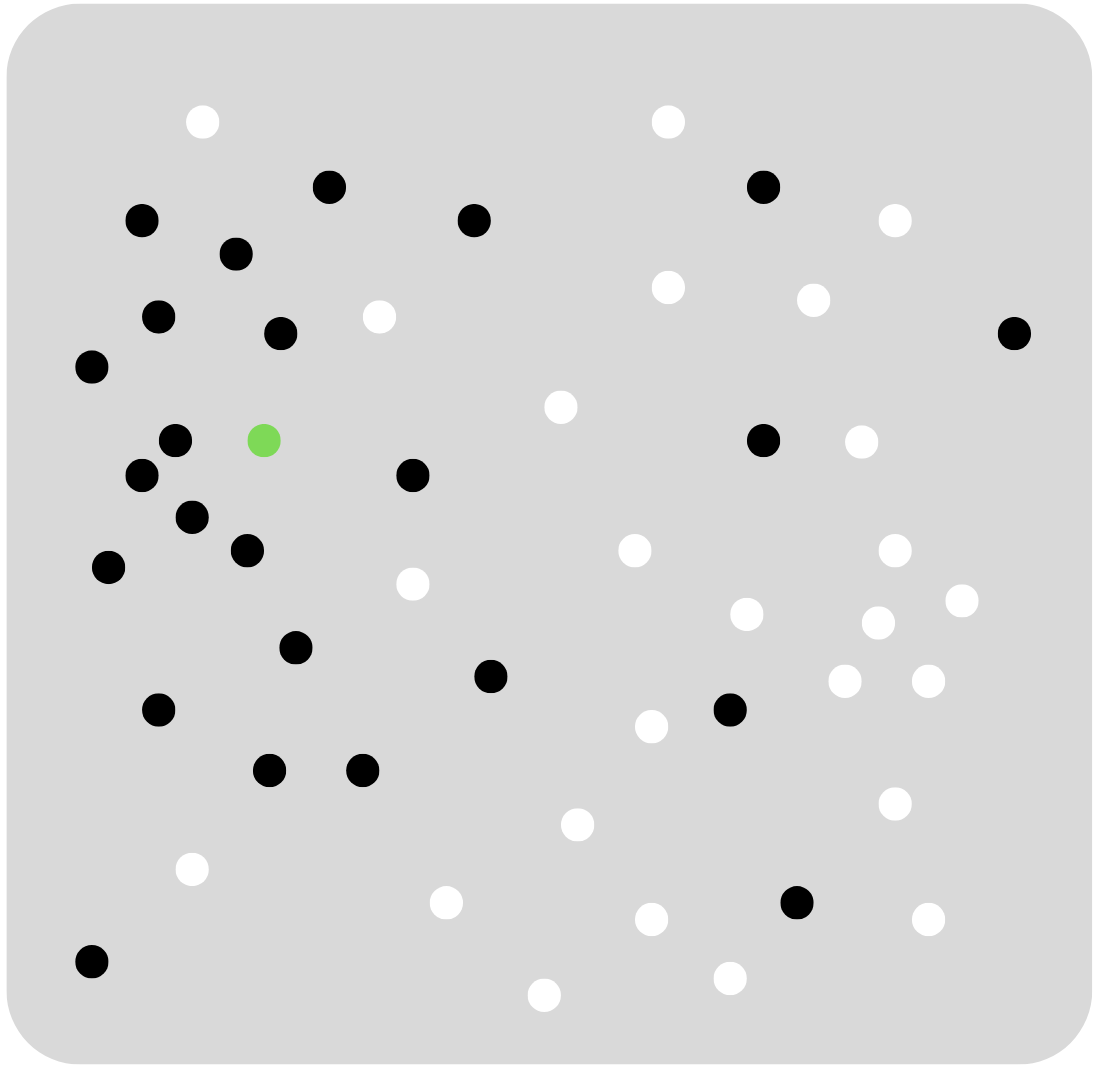
\includegraphics[width=0.2\textwidth]{vector_space/LLM_vector_space.png}
%   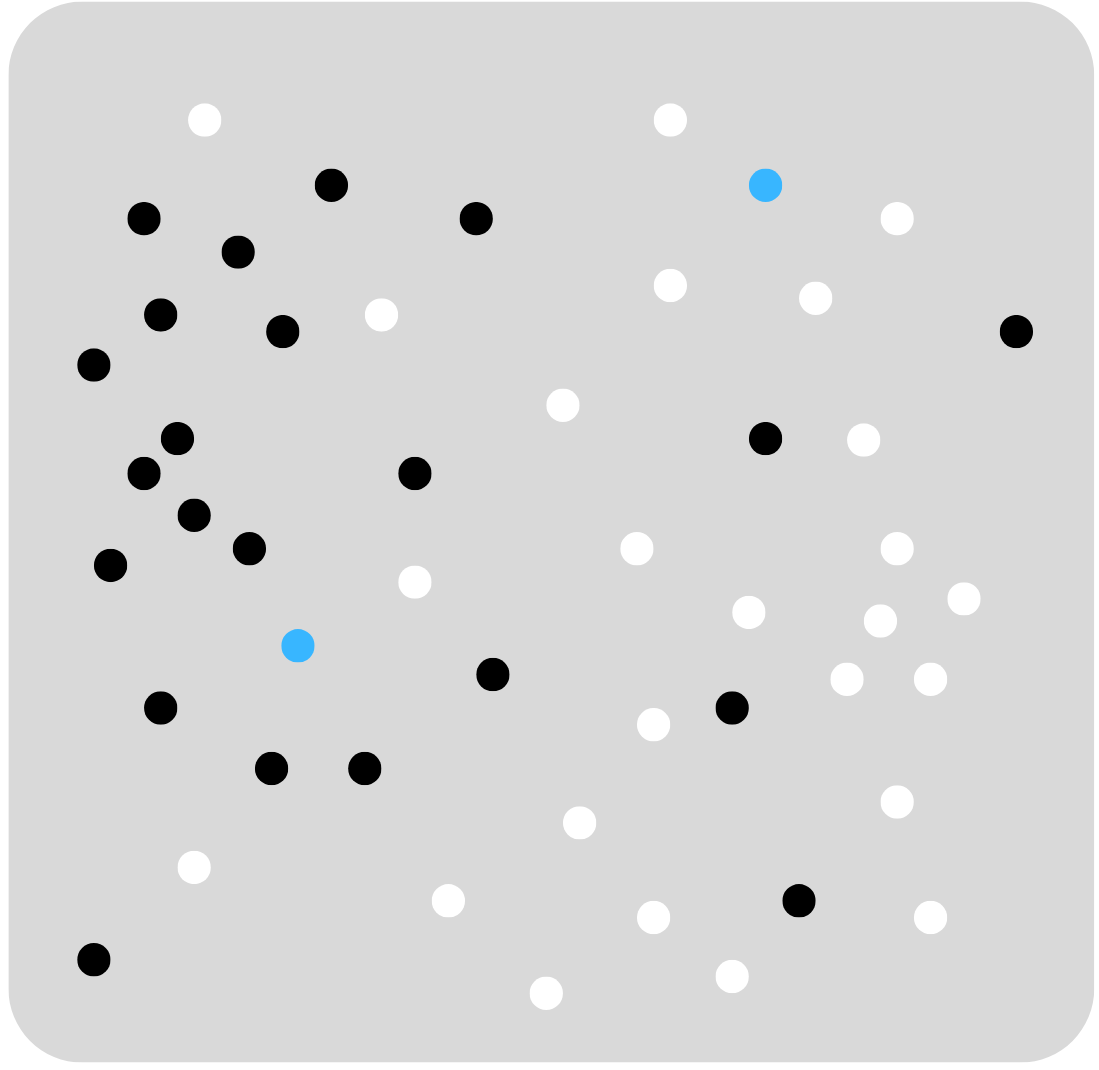
\includegraphics[width=0.2\textwidth]{vector_space/random_vector_space.png}
%   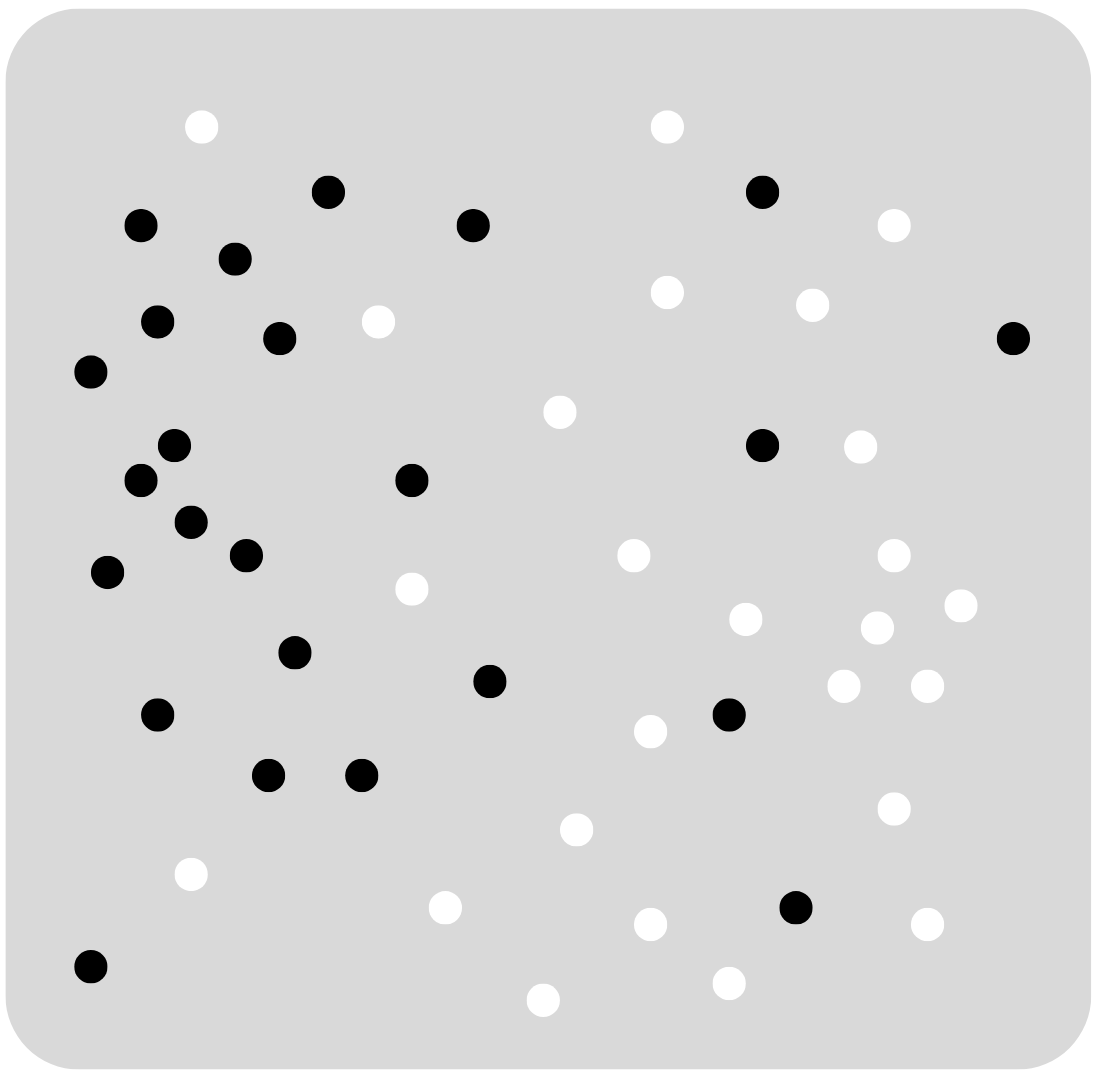
\includegraphics[width=0.2\textwidth]{vector_space/no_vector_space.png}
%   \caption{Ideal starting point for systematic reviews using active learning}
%   \label{fig:my-image}
% \end{figure}


% \subsubsection{Simulation design}

% In other words, whether, in the case of AI-assisted reviewing, prompt engineering actually aids in knowledge discovery or whether LLMs simply repackage existing knowledge.

% More LLM-specific variables were considered in advance (such as degree of jargon), however, because early simulations showed difference between the LLM- and criteria-based initialisation conditions, these variables were not further investigated. Future work may consider these variables in more detail.

% Most eligibility criteria are written in either conjunctive or disjunctive form. In the latter case, all the inclusion criteria must be met for a paper to be included, whereas in the former, only one must be met. This may affect how useful LLM-generated examples are compared to using the eligibility criteria directly or selecting random examples. This is because, for criteria in conjunctive form, abstracts will be relevant if and only if all the terms from the eligibility criteria are mentioned. In contrast, for criteria in in disjunctive form, the relevant abstracts will likely only contain one of the many terms mentioned in the eligibility criteria. 

% \subsubsection{Statistical Analysis}

% AI-assistant screening is actually sequence dependent. This is ignored by simply the summed successes and number of retrievals. Future work may consider modelling the sequence directly.

% The response variable makes sense to be viewed as a proportion and not a count because we know the true number of total relevant records. Future work modelling the retrieval of actual retrievals may more aptly consider it counts instead (e.g., Poisson).

% GLMM assume that the random effects are normally distributed (i.e., that the difference in starting performance between datasets follows a normal distribution). However, based on the results of a previous simulation study comparing the normalized loss performance of AI-assistant screening for different datasets, this seems unlikely \parencite{teijema2025large}. Future work may consider specifying a different random-effects distribution using hierarichal generalized linear models (HGLMs) or Bayesian methods.
% \subsection{Limitations}

% \begin{enumerate}
%     \item only one LLM used (gpt-4o-mini). Future work may consider other LLMs (e.g., open source LLMs).
%     \item Key limitation simulation study: data leakage (i.e., LLMs have been trained on synergy datasets). The ecological validity of the results are therefore somewhat limited.
%     \begin{enumerate}
%         \item There are two obvious solutions to the problem of data leakage: (1) apply the use of LLm-initialization on a new systematic review, and (2) use an older LLM from hugging face for example. 
%     \end{enumerate}
%     \item Another possible limitation: no switching of active leaning cycles (could fix contamination of synthetic data issue). 
%     \item The multilevel model assumption of heterogeneity between conditions may not hold. 
%     \item The effect of the length abstract may be small in part because this parameter had limited effect on the generated abstracts. However, since early analyses showed that the effect of the other LLM-specific parameters was limited (i.e., for temperature and number of abstracts), it is unlikely that the effect of length of abstract would be large either.
% \end{enumerate}

% Clusters should not be a problem because we only focus on starting performance (i.e., first 100 screened). Future work may consider the contamination hypothesis in more detail. 

\newpage

\appendix
\addcontentsline{toc}{part}{Appendix} % adds "Appendix" to table of contents
\part*{\Large Appendix}                       % prints "Appendix" as a unnumbered heading


\FloatBarrier
\section{SYNERGY metadata}

\begin{table} [h!]
\centering
\caption{SYNERGY datasets overview}
\label{tab:SYNERGY}
\begin{tabularx}{\textwidth}{@{}r l X r r r@{}}
\toprule
\textbf{Nr} & \textbf{Dataset} & \textbf{Topic(s)} & \textbf{Records} & \textbf{Included} & \textbf{\%} \\
\midrule
1  & Appenzeller-Herzog\_2019 & Medicine & 2873  & 26  & 0.9 \\
2  & Bos\_2018                 & Medicine & 4878  & 10  & 0.2 \\
3  & Brouwer\_2019             & Psychology, Medicine & 38114 & 62  & 0.2 \\
4  & Chou\_2003                & Medicine & 1908  & 15  & 0.8 \\
5  & Donners\_2021             & Medicine & 258   & 15  & 5.8 \\
6  & Hall\_2012                & Computer science & 8793  & 104 & 1.2 \\
7  & Leenaars\_2019            & Psychology, Chemistry, Medicine & 5812  & 17  & 0.3 \\
8  & Leenaars\_2020            & Medicine & 7216  & 583 & 8.1 \\
9  & Meijboom\_2021            & Medicine & 882   & 37  & 4.2 \\
10 & Menon\_2022               & Medicine & 975   & 74  & 7.6 \\
12 & Muthu\_2021               & Medicine & 2719  & 336 & 12.4 \\
13 & Nelson\_2002              & Medicine & 366   & 80  & 21.9 \\
14 & Oud\_2018                 & Psychology, Medicine & 952   & 20  & 2.1 \\
15 & Radjenovic\_2013          & Computer science & 5935  & 48  & 0.8 \\
16 & Sep\_2021                 & Psychology & 271   & 40  & 14.8 \\
17 & Smid\_2020                & Computer science, Mathematics & 2627  & 27  & 1.0 \\
18 & van\_de\_Schoot\_2018     & Psychology, Medicine & 4544  & 38  & 0.8 \\
19 & van\_der\_Valk\_2021      & Medicine, Psychology & 725   & 89  & 12.3 \\
20 & van\_der\_Waal\_2022      & Medicine & 1970  & 33  & 1.7 \\
21 & van\_Dis\_2020            & Psychology, Medicine & 9128  & 72  & 0.8 \\
22 & Walker\_2018              & Biology, Medicine & 48375 & 762 & 1.6 \\
23 & Wassenaar\_2017           & Medicine, Biology, Chemistry & 7668  & 111 & 1.4 \\
24 & Wolters\_2018             & Medicine & 4280  & 19  & 0.4 \\
\bottomrule
\multicolumn{6}{p{\textwidth}}{\footnotesize\textit{Note:} Three of the datasets included in the original SYNERGY dataset were excluded entirely due to data quality issues: Chou\_2004, Moran\_2021 and Jeyaraman\_2020.}
\end{tabularx}
\end{table}

\section{LLM generated abstracts}
\label{sec: LLM generated abstracts}

\begin{tcolorbox}[title=Eligibiltiy Criteria, colback=gray!10, colframe=gray!50, fontupper=\small]
To be eligible for inclusion in the SR sample, documents had to fulfil the following criteria:
\begin{enumerate}[leftmargin=*, nosep]
    \item identify explicitly as a "systematic review" in their title;
    \item assess the effect of a non-acute, non-communicable, environmental exposure on a health outcome;
    \item include studies in people or mammalian models;
    \item be available in HTML format;
    \item be published between 1 January 2019 and 30 June 2020.
\end{enumerate}
\end{tcolorbox}

\begin{tcolorbox}[title=LLM-generated Abstract, colback=gray!10, colframe=gray!50, fontupper=\small]
\textbf{title: }The Impact of Urban Air Pollution on Respiratory Health: A Systematic Review: \newline \textbf{abstract: }This systematic review evaluates the effects of urban air pollution, a significant non-acute, non-communicable environmental exposure, on respiratory health outcomes in human populations. Spanning studies published between January 2019 and June 2020, this review incorporates findings from various research articles available in HTML format, ensuring compatibility with blinding strategies. The analysis details how exposure to pollutants, including particulate matter and nitrogen dioxide, correlates with increased incidences of asthma, chronic obstructive pulmonary disease (COPD), and other respiratory ailments. The review synthesizes data from multiple cohorts, emphasizing the need for public health interventions to mitigate pollution's impact on vulnerable populations. We discuss the implications of these findings in the context of urban planning and policy-making, aiming to foster environments that protect respiratory health.
\end{tcolorbox}

% References
\FloatBarrier
\printbibliography
%TC:endignore

\end{document}




% \begin{tcolorbox}[title=Eligibiltiy Criteria, colback=gray!10, colframe=gray!50, fontupper=\small]
% The search was not limited by the year of publication. Journal papers and conference proceedings were included. The search was limited to English.

% During the systematic review, we included empirical studies validating and assessing software metrics in the area of software fault prediction. For the selection of primary studies, the following
% inclusion and exclusion criteria were used. Inclusion criteria:
% Empirical studies (academic and industry) using large and small scale data sets AND.
% Studies comparing software metrics performance in the area of software fault prediction.

% Exclusion criteria:
%  Studies without an empirical validation or including experimental results of software metrics in fault prediction OR.
% Studies discussing software metrics in a context other than software
% fault prediction (e.g. maintainability) OR.
% Studies discussing modeling techniques (e.g. Naive Bayes, Random
% Forest) and not software metrics.
% Studies discussing and comparing prediction techniques were
% excluded from the review,
% Studies proposing new software metrics and not empirically
% validating them were also excluded
% \end{tcolorbox}




% \section{Format exported simulation results} \label{sec:format_exported_simulation_results}

% Each simulation run is stored in a separate CSV file. Every row represents a screened paper and contains the following information:

% \begin{enumerate}[label=\arabic*), leftmargin=*, nosep]
%   \item The paper's record ID,
%   \item The assigned label (i.e., relevant or irrelevant),
%   \item The classifier, querier, balancer and feature extractor used,
%   \item The size of the training set,
%   \item A time tag.
% \end{enumerate} 

% Furthermore, the following naming convention is used for the CSV files: \newline condition\_run\_run\_IVs\_n\_abstracts\_length\_abstracts\_llm\_temperature.csv. The same naming convention is used for the recall plots of each simulation run and for the generated abstracts in the LLM initialisation condition.

% Finally, at the end of each run, the current values of the input parameters, the outcome variables and other relevant metadata are appended to a long format master dataframe for analysis. The columns of this dataframe are as follows:

% \begin{enumerate}[label=\arabic*), leftmargin=*, nosep]
%     \item the name of the outcome variable
%     \item the value of the outcome variable
%     \item name of the simulated dataset,
%     \item the condition,
%     \item the values of the independent variables (NaN for the control conditions):
%         \begin{enumerate}
%         \item number of abstracts
%         \item length of the abstracts
%         \item temperature settings of the llm (i.e., diversity)
%         \end{enumerate}
%     \item timestamp
%     \item the run number
% \end{enumerate}

% This yields a data-frame containing one observation for each combination of dataset (n=26), condition (n=3), independent variables and their levels (n=$3 \times 4 \times 4 \times 5 \times 5 = 1200$), and run (n=1), thus with $26 \times 3 \times 1200 \times 1 = 93600$ rows, and the 12 columns enumerated above. 

% \section{Padding} \label{sec:padding}

% It is worth noting that the simulation may stop prematurely if all the relevant records are found before the stopping rule is reached (e.g. after screening 100 records). To accurately emulate a researcher who is unaware that all the relevant records have been found and therefore continues screening until the stopping rule is reached, the simulation results were supplemented with rows containing the label 'zero' (i.e. irrelevant records) until the stopping rule would have been reached. This process is referred to as 'padding' and ensures that the final simulation results are accurate.
